\documentclass[varwidth=true, border=2pt]{standalone}

\usepackage{pgfplots}
\usepackage{tikz}
\usetikzlibrary{arrows, positioning, calc}

\begin{document}
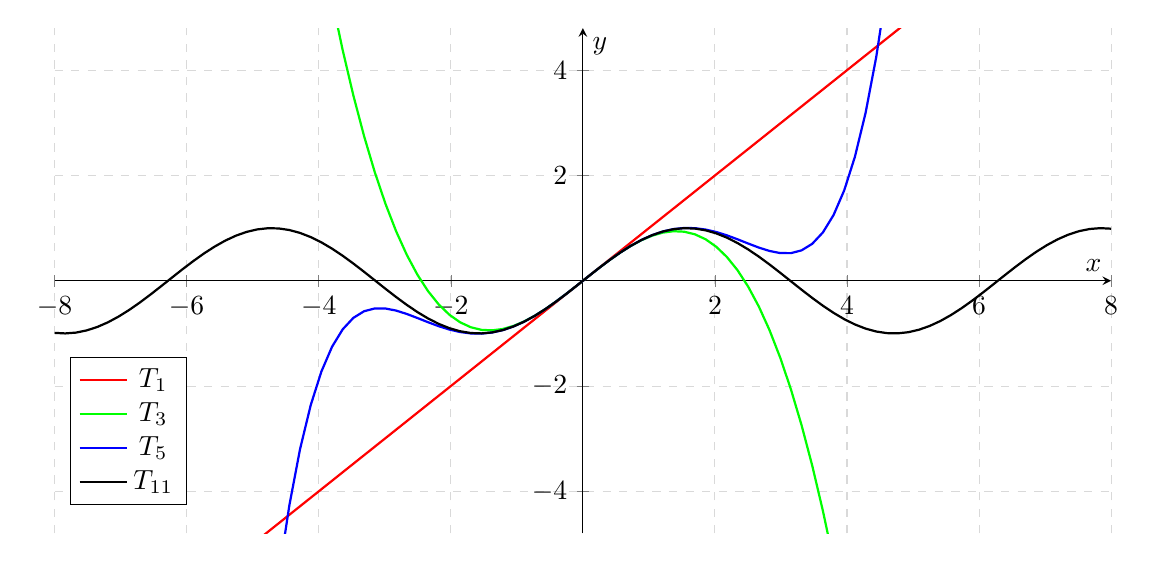
\begin{tikzpicture}
    \begin{axis}[
        axis x line=middle,
        axis y line=middle,
        enlarge y limits=true,
        xmin=-8, xmax=8, % Positive domain...
        width=15cm, height=8cm,     % size of the image
        grid = major,
        grid style={dashed, gray!30},
        ymin=-4,      % start the diagram at this y-coordinate
        ymax= 4,      % end   the diagram at this y-coordinate
        axis background/.style={fill=white},
        ylabel=$y$,
        xlabel=$x$,
        legend style={at={(0.07,0.35)}, anchor=north}
     ]
      \addplot[domain=-8:8,thick,samples=100,red] {x};
      \addplot[domain=-8:8,thick,samples=100,green] {x-x^3/6};
      \addplot[domain=-8:8,thick,samples=100,blue]  {x-x^3/6+x^5/120};
      %\addplot[domain=-8:8,thick,samples=100,pink]  {x-x^3/6+x^5/120-x^7/5040+x^9/362880-x^11/3916800};
      \addplot[domain=-8:8,thick,samples=100,black] {sin(deg(x))};
      \legend{$T_1$, $T_3$, $T_5$, $T_{11}$, $T_\infty$}
    \end{axis} 
\end{tikzpicture}
\end{document}
